\documentclass[a4paper,11pt]{article}
\usepackage{amsmath,amssymb,amsthm}

\usepackage[T1]{fontenc}
\usepackage[utf8]{inputenc}
\usepackage[english]{babel}
\usepackage{kpfonts}
\usepackage[autostyle]{csquotes}
\usepackage{mathrsfs}
\usepackage[style=alphabetic,backend=biber]{biblatex}
\addbibresource{References.bib}
\usepackage{hyperref}
\usepackage{braket}


\usepackage{graphicx}
\usepackage{caption}
\usepackage{subfig}
%\usepackage{subcaption}
%\usepackage[export]{adjustbox}


\theoremstyle{plain}
\newtheorem{theorem}{Theorem}[section]
\newtheorem{lemma}[theorem]{Lemma}
\newtheorem{prop}[theorem]{Proposition}
\newtheorem*{cor}{Corollary}
\newtheorem*{ex}{Exercise}

\theoremstyle{definition}
\newtheorem{defn}[theorem]{Definition}
\newtheorem{exmp}[theorem]{Example}

\theoremstyle{remark}
\newtheorem*{rem}{Remark}

\newcommand{\N}{{\mathbb N}}
\newcommand{\Z}{{\mathbb Z}}
\newcommand{\C}{{\mathbb C}}
\newcommand{\Q}{{\mathbb Q}}
\newcommand{\R}{{\mathbb R}}
\newcommand{\F}{{\mathbb F}}
\newcommand{\K}{{\mathbb K}}
\renewcommand{\L}{{\mathbb L}}
\newcommand{\sdir}{\mathbb{o}}
\newcommand{\nil}{\mathfrak N}
\newcommand{\abs}[1]{\lvert#1\rvert}
\newcommand{\norm}[1]{\left\lVert#1\right\rVert}
\renewcommand{\epsilon}{\varepsilon}

\DeclareMathOperator{\Norm}{\mathfrak{N}}
\DeclareMathOperator{\Trace}{\mathfrak{T}}
\DeclareMathOperator{\Aff}{Aff}
\DeclareMathOperator{\GL}{GL}
\DeclareMathOperator{\dist}{\mathfrak{d}}
\DeclareMathOperator{\U}{U}
\DeclareMathOperator{\LL}{L}
\newcommand{\xq}[1]{X_q (\delta ,#1)}
\newcommand{\rd}{\sqrt{\delta}}
\DeclareMathOperator{\I}{I}
\DeclareMathOperator{\A}{A\!}

\begin{document}
\author{Lorenzo Baldi, Salvatore Schiavulli}
\title{Discrete Fourier Analysis report}
\maketitle
\tableofcontents\section{Introduction}
This report is divided in two main parts: in the first, more abstract, we developed representation theory of finite 
(even non abelian) groups; in the second we studied some kind of graphs over the finite upper half plane, that is a subset of
certain finite fields. The main reference is our textbook \cite{terras_1999}, in particular chapters 
(mettere qui i capitoli che hai usato) for the part of representation theory and chapter 18 for the second part.
Our work was studying and filling the gaps (examples and proofs left as exercises) in these chapters. It was not easy,
since the exposition is very strict and many proofs are just sketched or omitted with a link to a reference. In any case,
especially in the first part, we had to skip some details and proofs for reason of space, in order to reach the 
theorems we needed for the second part.

Mettere qua le giustificazioni per cui rappresentazione di gruppi è interessante.

In the second part we had the chance to develop and apply the theory of finite fields
to a concrete example. This lead us to some concepts (e.g. absolutely irreducibility, number of solutions of certain equations)
that we can find also in the theory of elliptic curves. In fact we find an equation of the form $x^2=f(y)$.
Moreover we wrote a MAGMA program that allowed us to compute some characteristic of the graphs we where analyzing, to have 
the felling of what was happening, and we used SAGE to plot these graphs for small number of vertexes.

\section{Representations of finite groups}
In this report $\F_q$ indicates the finite field with $q=p^r$ elements, where $p$ is a prime and $r$ is an integer greater then zero.

Here we are interested in doing Fourier analysis on some subgroups of the \emph{General linear group}, which is defined below. 
\begin{defn}
The {\it General Linear group} of dimension $n$ over the field $\F_q$ is the group of $n\times n$ invertible matrices with entries in $\F_q$:
\begin{equation*}
\GL(n,\F_q)=\Big\{ A \in \F_q^{n \times n} \colon \det A = \abs A\neq 0 \Big\}.
\end{equation*}	
\end{defn}
In particular we will focus on $GL(2,\F_q)$ and on its subgroup $\Aff(q)$, \emph{i.e.}, the \emph{Affine group}:
\begin{defn}
The {\emph{ Affine group}} of dimension two over the field $\F_q$ is:
\begin{equation}
\label{def:aff_group}
\Aff (q)=\Big\{ A=\begin{pmatrix} a & b \\ 0 & 1 \end{pmatrix}\in \GL(2,\F_q) \Big\}=\Big\{ A=\begin{pmatrix} a & b \\ 0 & 1 \end{pmatrix} \colon a,b \in \F_q, \, a \neq 0 \Big \}.
\end{equation}
\end{defn}
Since we want to do Fourier analysis on these groups, first of all we must map them (homomorphically) into groups of complex matrices. To do that we need to introduce the concept of representation of a finite group $G$.

\begin{defn}
A (finite dimensional) representation of a finite group $G$ is a group homomorphism
\[
\pi:  G \rightarrow \GL(n,\C).
\]
If, for $g\in G$, $\pi(g)$ is a matrix with $i,j$ entry $\pi_{i,j}(g)$, we call the functions $\pi_{i,j} : G \rightarrow \C$ the \emph{matrix entries} of $\pi$.
\end{defn}
\begin{rem}
We can identify $\GL(n,\C)$ and
\[
\GL(V)=\{T\colon V\rightarrow V \ | \  T \text{ is linear and invertible}\},
\]
where $V$ is an $n$-dimensional vector space over $\C$. However notice that in this case the matrix entries $\pi_{i,j}$ change if change the basis of $V$ and this can cause some issue. In any case, will use the two concepts interchangeably.
\end{rem}

We give now some important definition about representations. In the following $G$ indicates a finite group.
\begin{defn}
\label{equiv:repres}
To representations $\alpha$ and $\beta$ of $G$ into $\GL(n,\C)$ are said to be \emph{equivalent}
if there exists a matrix $T \in \GL(n,\C)$ such that
\[
T\alpha(g)T^{-1}=\beta(g), \quad \forall g \in G.
\]
This is equivalent to say that we can obtain one representation from the other by a uniform change of basis.
\end{defn}

\begin{defn}
\label{def:unitary}
A \emph{unitary} representation is a representation $\pi$ which maps $G$ into the unitary group $\U(n)$, where 
\[
\U(n) =\{A\in \GL(n,\C) \colon {}^{t}\!\bar{A}A=I\}.
\]
\end{defn}
\begin{rem}
If $\Braket{u, \, v} = {}^t\!\bar{u}v$ is the standard Hermitian inner product of vectors of $\C^{n}$, the unitary matrices are those which preserve this product, that is, $\Braket{Au, \, Av} =\Braket{u, \, v} \ \forall u,v \in \C^{n}$.
Indeed, if $A \in \U(n)$, then by the definition of the inner product, we have $\Braket{Au, \, Av}={}^{t}\!\overline{(Au)}Av={}^t\!\bar{u}{}^t\!\bar{A}Av={}^t\!\bar{u}v=\Braket{u,\, v} \ \forall u,v \in \C^{n}$ and vice versa if $\Braket{Au, \, Av} =\Braket{u, \, v} \ \forall u,v \in \C^{n}$ then, by taking $u_i=(0,\dots ,0, 1, 0,\dots , 0)$ where the $1$ is in the $i$-$th$ coordinate, we see that, indicating with $a_i$ the $i$-$th$ column of $A$, $\delta_{i,j}=\langle u_i, \, u_j\rangle =\langle Au_i, \, Au_j\rangle={}^t\!\bar{a_i}a_j$, that is ${}^{t}\!\bar{A}A=I$.
\end{rem}
\begin{defn}
A \emph{subrepresentation} $\rho$ of a representation $\pi\colon G \rightarrow \GL(V)$ means that $\rho\colon G \rightarrow \GL(W)$, where $W$ is a subspace of $V$ such that $\pi(g)W\subset W \text{ for all }g \in G$ and $\rho(g)$ is the restriction of $\pi(g)$ to $W$, \it{i.e.}
\[
\pi(g)_{\mkern 1mu \vrule height 2ex\mkern2mu W}= \rho(g)\ \forall g \in G
\]
Using matrix language, this means that there is a basis of $V$ such that $\pi(g)$ has the block form:
\[
\begin{pmatrix}
\rho(g) & \ast \ \\
0 & \ast \
\end{pmatrix}
\]
\end{defn}
\begin{defn}
A representation  $\pi$ is \emph{irreducible} if its only subrepresentations are $\pi$ itself and 0.
\end{defn}
When we deal with representations of a finite group $G$, we can just consider the unitary ones, due to the following result:
\begin{prop}
\label{unit:eqiv}
If $G$ is a finite group, every representation is equivalent to a unitary representation.
\end{prop}
\begin{proof}[Proof sketch.]
To prove this preposition we'll use the fact (which we aren't going to prove) that if a matrix $M$ leaves invariant some positive definite, Hermitian inner product $c(u,v)$ for $u,v \in \C^n$, then $M$ is conjugate to a unitary matrix.
So it suffices to find an inner product which is invariant under $\pi(g)$ for all $g \in G$. Such a inner product is given by 
\[
c(u,v)= \sum_{g \in G} \Braket{ \pi(g)u, \pi(g)v } , \text{ for } u,v \in \C^n,
\]
as one can easily check.
%Indeed, for $h\in G$, $u,v\in \C^n$, we have
%
%\[
%\begin{split}
%c(\pi(h)u,\pi(h)v) &= \sum_{g \in G} \Braket{ \pi(g)\pi(h)u, \pi(g)\pi(h)v } \\
%&=\sum_{g \in G} \Braket{ \pi(gh)u, \pi(gh)v } \\
%&=\sum_{k \in G} \Braket{ \pi(k)u, \pi(k)v }= c(u,v).\\
%\end{split}
%\]

Where we have made the substitution $gh=k$, so that if $h$ runs through all the elements in $G$, so does $k$. 
\end{proof}
Let us now introduce  the space of functions from $G$ to $\C$ 
\begin{equation*}
\LL^2(G)=\Set{f\colon G \rightarrow \C},
\end{equation*}
which is a vector space over $\C$ of dimension $\abs G$ (it is isomorphic to $\C^n$, with $n=\abs G$).
We can make $\LL^2(G)$ an algebra by defining the \emph{convolution} $a\ast b$, for $a,b\in \LL^2(G)$, $x\in G$:
\begin{equation*}
(a\ast b)(x)=\sum_{t \in G} a(xt^{-1})b(t)=\sum_{y \in G} a(y)b(y^{-1}x)
\end{equation*}
\begin{rem}[non necessario]
This definition of convolution coincides with that given for the commutative group $\Z/{n\Z}$ ($(a\ast b)(x)=\sum_{y \in \Z/{n\Z}} a(y)b(x-y)$). 
Moreover we have that, given $f\in \LL^2(G)$,
\begin{equation}
\label{conv:comm}
f*h=h*f \quad \forall h \in \LL^2(G)
\end{equation}

if and only if $f$ is constant on conjugacy classes
\[
\Set{g}=\Set{xgx^{-1}\colon x\in G}.
\]
Indeed if $f$ is constant on conjugacy classes, then for all $x\in G$
%\[
\begin{multline*}
(f\ast h)(x) =\sum_{t \in G} f(xt^{-1})h(t)=\sum_{xt \in G} f(x(xt)^{-1})h(xt)\\
=\sum_{xt \in G} f(xt^{-1}x^{-1})h(xt)
=\sum_{xt \in G} f(t^{-1})h(xt)
=\sum_{y \in G} f(y^{-1}x)h(y)= (h*f)(x),
\end{multline*}
%\]
and, conversely, if \ref{conv:comm} holds, then, taking $h=\delta_k$, for $k\in G$, we have that $(f\ast h)(ky)=f(kyk^{-1})$ and $(h*f)(ky)=f(y)$ for all $y \in G$, so that $f$ is constant on conjugacy classes.
Since if $G$ is commutative the conjugacy class $\{g\}$ contains only $g$, it follows that the convolution is commutative for abelian groups, as we already know.
\end{rem}
\begin{exmp}
\label{exa:lrr}
We define the \emph{Left Regular Representation} $L$ of $G$ by 
\begin{align*}
L\colon G &\rightarrow \GL(\LL^2(G))\\
	 g&\mapsto L(g) 
\end{align*}
where 
\[
[L(g)a](x)=a(g^{-1}x)
\]
for $a \in \LL^2(G)$ and $x,g \in G$.
We have to check that the function $L$ defined above is indeed a group representation, that is, we have to check $L(xy)=L(x)L(y)$ for all $x,y \in G$. Let's take $a \in \LL^2(G)$ and $g\in G$, then
\[ [L(xy)a](g)=a((xy)^{-1}g)=a(y^{-1}x^{-1}g)
\]
and
\[
[L(x) L(y)a](g)=[L(x)(L(y)a)](g)=[L(x)b](g)=b(x^{-1}g)=a(y^{-1}x^{-1}g),
\]
where $b=L(y)a \in \LL^2(G)$.

Fix now $g\in G$, we want to write the matrix of $L(g)$ in the basis of $\LL^2(G)$ consisting of delta functions $\delta_g(x)=1$ if $x=g$ and 0 otherwise. For all $h,x\in G$, we have $[L(g)\delta_h](x)=\delta_h(g^{-1}x)=1 \iff g^{-1}x=h \iff x=gh$, so that $L(g)\delta_h=\delta_{gh}$. Thus if we write $G=\{g_1,g_2,\dots , g_n\}$ we have that the $j$-th column of $L(g)$ is $([L(g)\delta_{g_j}](g_1),\dots [L(g)\delta_{g_j}](g_n))=(\delta_{gg_j}(g_1),\dots \delta_{gg_j}(g_n))=$, but then we have $\delta_{gg_j}(g_i)=1\iff g_i=gg_j\iff g=g_ig_j^{-1}$ and so we can conclude that the $i,j$ entry of $L(g)$ is $\delta_{g_ig_j^{-1}}(g)$. This means that in every row and in every column of $L(g)$ there is only one entry equal to 1 and all the others are zero. So $L(g)$ is obtained from the identity matrix by a permutation of its rows (or columns). Note that if $g$ is not the identity element $e$ of $G$, then $L(g)_{ii}=\delta_{g_ig_i^{-1}}(g)=\delta_{e}(g)=0$.
\end{exmp}

Now we want to decompose a representation $\pi$ of $G$ into irreducible part, \textit{i.e.}, considering $\pi$ as a matrix, we want to replace $\pi$ by a matrix which has diagonal blocks that cannot be further decomposed. This is achieved by the following proposition.
Note that by \ref{unit:eqiv} we can assume all representations are unitary.
\begin{prop}[Complete Reducibility Theorem]~ 
\label{thm:complred}
\begin{enumerate}
\item Suppose that $\rho\colon G\rightarrow \U(m)$ is a subrepresentation of the representation $\pi\colon G\rightarrow \U(n)$. Then $\pi$ is equivalent to the representation with block diagonal form:
\[(\rho \oplus \sigma)(g)=
\begin{pmatrix}
\rho(g) & 0 \\
0 		& \sigma(g)
\end{pmatrix}.
\]
\item By induction, $\pi(g)$ is equivalent to
\[
(\pi_1(g)\dots \pi_r(g))= 
\begin{pmatrix}
\pi_1(g)  &{} &0\\
{} &\ddots &{} \\
0 &{}  &\pi_r(g)
\end{pmatrix},
\]
where each subrepresentation $\pi_i$  is irreducible. we say, when this happens, that $\pi$ is \emph{completely reducible}. 
\end{enumerate}
\end{prop}
\begin{proof}~ 
\begin{enumerate}
\item We know that, by the remark after definition \ref{def:unitary}, if $\pi(g)$ is unitary then it leaves invariant the standard inner product $\braket{u,\, v}={}^t\!\bar{u}v$ for $u,v \in \C^n$. Moreover, since $\rho$ is a subrepresentation of $\pi$, by definition there is a subspace $W$ of $V=\C^n$ such that $\pi(g)W\subset W$ and, for all $g\in G$, $\pi(g)_{\mkern 1mu \vrule height 2ex\mkern2mu W}= \rho(g)$.  Consider the \emph{orthogonal complement space} $W^\perp$ of $W$:
\[
W^{\perp}= \Set{v \in V \colon \braket{u, \, v}=0 \text{ for all } w \in W}.
\]
Then we claim that $\pi(g)W^{\perp}\subset W^{\perp}$. Indeed, take $w\in W^{\perp}$, then, for all $v\in W$, we can write (since $\pi(g) \in \GL(n,\C)$) $v=\pi(g)v'$, where $v'=\pi(g)^{-1}v=\pi(g^{-1})v \in W$. Then we have 
\[
\braket{\pi(g)w,\, v}=\braket{\pi(g)w,\, \pi(g)v'}=\braket{w,\, v'}=0.
\]
And so $\pi(g)w\in W^{\perp}$. This means that the restriction $\pi(g)_{\mkern 1mu \vrule height 2ex\mkern2mu W^{\perp}}= \sigma(g)$ is a subrepresentation of $\pi$.  Then, since we are working in $\C^n$, we can just take a basis of $V$ consisting in a combination of a basis of $W$ and a basis of $W^{\perp}$. If we write $\pi(g)$ in this basis we obtain exactly the matrix given in the statement of the proposition.
\item This follows easily by induction on $n$.
\end{enumerate}
\end{proof}

The next lemma, due to Issai Schur, is crucial to do Fourier analysis on finite groups.

\begin{lemma}[Schur's Lemma].
Suppose that $\pi\colon G\rightarrow \GL(V)$ and $\rho\colon G\rightarrow \GL(W)$ are representations of $G$. We define the space $\I(\pi,\rho)$ of the \emph{intertwining operators} between $\pi$ and $\rho$ as follows
\[
\I(\pi,\rho)=\Set{L\colon V\rightarrow W | L \text{ is linear and } L\circ \pi(g)= \rho(g)\circ L , \ \forall g\in G}.
\]
Suppose $L\in \I(\pi,\rho)$, then the following hold:
\begin{enumerate}
\item The restriction of $\pi$ to $\ker(L)$ is a subrepresentation of $\pi$ and  the restriction of $\rho$ to $\Im(L)$ is a subrepresentation of $\rho$.
\item If $\pi$ and $\rho$ are both irreducible representations and $L$ is not the null map, then $L$ is an isomorphism between $V$ and $W$ (and so $\pi$ and $\rho$ are equivalent).
\item If $\pi$ is irreducible and $L\in \I(\pi,\pi)$,  then $\exists \lambda \in \C$ such that $Lv=\lambda v$, for all $v\in V$, \emph{i.e.}, $L=\lambda I$, where $I$ is the identity operator.
\item If both $\pi$ and $\rho$ are irreducible, then 
\[
\dim_\C\I(\pi, \rho)=
\begin{cases}
1 &\text{if $\pi$ and $\rho$ are equivalent,} \\
0 &\text{otherwise.}
\end{cases}
\]
\end{enumerate}
\end{lemma}
\begin{proof}~ 
\begin{enumerate}
\item Let $v \in \ker(L)$, then 
\[
L(\pi(g)v)=\rho(g)(Lv)=\rho(g)0=0, \quad \forall g\in G,
\]
so that $\pi(g)v\in \ker(L)$.

Analogously if $w \in \Im(L)$, then $w=Lv$ for some $v\in V$, thus
\[
\rho(g)w=\rho(g)(Lv)=L(\pi(g)v)\in \Im(L), \quad \forall g\in G.
\]


\item Since $L\neq 0$, we have $\ker(L)\neq V$, so by 1. and the fact that $\pi$ is irreducible, this means $\ker(L)=\{0\}$. Analogously, since $L\neq 0$, we have $\Im(L)\neq 0$, that is, using again 1. and the fact that $\rho$ is irreducible, $\Im(L)=W$. So $L$ is bijective.
\item Since we are working on $\C$, there exist a root $\lambda$ of $\det(xI-L)$, that is, an eigenvalue of $L$. Denote with $V_\lambda$ the eigenspace corresponding to the eigenvalue $\lambda$:
\[
V_\lambda=\Set{v\in v \colon Lv=\lambda v}\neq \{0\}.
\] 
Then $\pi(g)(V_\lambda)\subset V_\lambda$, since $L(\pi(g)v)=\pi(g)(Lv)=\pi(g)(\lambda  v)=\lambda\pi(g) v$, and so $\pi(g)v\in V_\lambda$. This means that the restriction of $\pi$ to $V_\lambda$ is a subrepresentation of $\pi$, which is irreducible, thus $V_\lambda = V$ and this implies $L=\lambda I$ on $V$. 
\item Since every $\I(\pi,\rho)\ni L\neq 0$ is an isomorphism between $V$ and $W$ by point 2., if $\pi$ and $\rho$ are not equivalent, such an isomorphism cannot exist, and so $\I(\pi,\rho)=\{0\}$. Assume then that $\pi$ and $\rho$ are equivalent and consider $K,L\neq 0$ in  $\I(\pi,\rho)$. By point 2. $L$ is an isomorphism, so we can consider the map $M=L^{-1} \circ K\colon V\rightarrow V$. Since both $K$ and $L$ (and so $L^{-1}$) are nonnull, $M$ is a nonzero element of $\I(\pi,\pi)$. Then by 3. we have that there exists $0\neq \mu\in \C$ such that $M=\mu I$, \emph{i.e.} $K=\mu L$ and the dimension of $\I(\pi,\rho)$ is 1.
\end{enumerate}

\end{proof}
\begin{defn}
Let $\pi\colon G \rightarrow \GL(V)$ be a representation. We define the \emph{degree} $d_{\pi}$ (or dimension) of $\pi$ to be the dimension of the vector space $V$.
\end{defn}
\begin{cor}
Every irreducible representation of an abelian group $G$ must have degree 1.
\end{cor}
\begin{proof}
See \cite[p. 249]{terras_1999}.
\end{proof}
To do Fourier analysis on a finite group $G$ we will need a list of all inequivalent representation of $G$.

\begin{defn}
Let $G$ be a finite group, we denote with $\hat{G}$ a complete set of irreducible unitary representation of $G$.
\end{defn}
\begin{rem}
Note that every two one-dimensional representations must be inequivalent. This is because if $\pi$ is one-dimensional, then $\pi(G)$ is an element of $\C$ and so if $\rho$ is an equivalent representation, then by definition \ref{equiv:repres}, there exists $T\in \C$ such that $\rho(g)=T\pi(g) T^{-1} = TT^{-1}\pi(g)=\pi(g)$, for all $g\in G$.
\end{rem}
\begin{exmp}
\label{exa:characters}
$G=\Z/n\Z$ under addition modulo $n$.

In this case we have that $e_a(x)=\exp(2\pi iax/n)$ for $a,x\in G$ are one-dimensional representation of $G$, also called \emph{characters} of $G$. We will see (maybe) that $\hat{G}=\{e_a\colon a \in G\}$. 
\end{exmp}
\begin{defn}
Given a representation $\pi$ of $G$ we define the \emph{character} of $\pi$ as $\chi_\pi(g)=\text{Tr}(\pi(g))$, for all $g \in G$, where Tr($\pi(g)$) is the trace of the matrix $\pi(g)$.
\end{defn}
\begin{rem}
Note that $\chi_\pi(g)\colon G\rightarrow \C$, so if $\pi$ is one-dimensional, its character coincides with $\pi$ itself. Moreover, by definition we have $\chi_{\pi\oplus\rho}=\chi_{\pi} + \chi_\rho$.
\end{rem}
\begin{theorem}[Schur's Orthogonality Relations]~ 
\label{thm:schurel}
\begin{enumerate}
\item Suppose $\pi\colon G\rightarrow \U(n)$ and $\rho\colon G\rightarrow \U(m)$ are two inequivalent irreducible unitary representations of $G$. Then, using the standard inner product of $\LL^2(G)$, we have that the matrix entries of $\pi$ and $\rho$ are pairwise orthogonal:
\[
\braket{\pi_{ij},\, \rho_{rs}}=\sum_{g\in G}\pi_{ij}(g)\overline{\rho_{rs}(g)}=0, \quad \text{for all $i,j,r,s.$}
\]
\item if $\pi$ is as above, then 
\[
\braket{\pi_{ij},\, \pi_{rs}}=\frac{\abs G}{d_\pi}\delta_{ir}\delta_{js}.
\]
\item Let $\pi$ and $\rho$ be two irreducible unitary representations of $G$. Then the characters of $\pi$ and $\rho$ are also orthogonal, in particular we have:
\[
\braket{\chi_\pi,\, \chi_\rho}=
\begin{cases}
0 &\text{if $\pi$ and $\rho$ are inequivalent} \\
\abs G &\text{otherwise}
\end{cases}
\]
\end{enumerate}
\end{theorem}
\begin{proof}~ 
\begin{enumerate}
\item Consider an $n\times m$ complex matrix $C$, then define
\begin{equation*}
P=\sum_{g\in G}\pi(g)C\rho(g^{-1}),
\end{equation*}
which is also an $n\times m$ matrix. We have that $P\in \I(\pi, \, \rho)$, since
\[
\pi(g)P=\sum_{g \in G}\pi(hg)C\rho(g^{-1})=\sum_{g\in G}\pi(u)C\rho(u^{-1}h)=P\rho(h).
\]
were we have made the substitution $u=hg$ and  used the fact that both $\pi$ and $\rho$ are homomorphism. For point 2. of Schur's lemma we must have (since $\pi$ and $\rho$ are inequivalent) $P=0$. Now choose $C=E_{js}$, the matrix which is 1 in the $j,s$ entry and 0 elsewhere. This choice of $c$ forces the $i,r$ entry of $P$ to be 
\[
P_{ir}=\sum_{g\in G}\pi_{ij}\overline{\rho_{rs}(g)}=0.
\]
\item Analogously to the previous point we define 
\begin{equation}
\label{P:equation}
P=\sum_{g\in G}\pi(g)C\pi(g^{-1}), \quad \text{for any $n\times n$ matrix $C$.}
\end{equation}

By 3. of Schur's lemma, we have $P=\lambda_CI$, for some $\lambda_C\in \C$. Then, taking the trace in \ref{P:equation} we obtain
\[
\text{$\sum_{g\in G}$Tr$(C)=$Tr$(P)=$Tr$(\lambda_CI)=\lambda_C$Tr$(I)=\lambda_C\sum_{i=1}^n 1=\lambda_Cn=\lambda_Cd_\pi.$}
\]  
Where we have used the facts that the trace is linear and it satisfies the \emph{cyclic property} (for all $A,B,C$ matrices we have Tr$(ABC)=$Tr$(BCA)$). So we obtain $\lambda_C=\abs G \text{Tr$(C)d_\pi^{-1}$}$. Now we set $C=E_{js}$, as before, and obtain 
\[
\braket{\pi_{ij},\, \pi_{rs}}=\sum_{g\in G}\pi_{ij}(g)\overline{\pi_{rs}(g)}=P_{ir}=\frac{\abs G}{d_\pi}\delta_{ir}\delta_{js}.
\]
\item This follows from the previous points. Indeed if $\pi$ and $\rho$ are inequivalent, then by 1. and the definition of character we have
\[
\braket{\chi_\pi,\, \chi_\rho}=\braket{\sum_{i=1}^n\pi_{ii},\, \sum_{j=1}^n\rho_{jj} }=\sum_{i,j}\braket{\pi_{ii},\, \rho_{jj} }=0
\]
If $\rho$ and $\pi$ are equivalent, we can assume $\rho=\pi$. Indeed if $\rho$ and $\pi$ are two equivalent representations of $G$, then there exist  an invertible matrix $T$ such that $\pi(g)=T\rho(g)T^{-1}$, for all $g\in G$. Thus by definition of character and by the cyclic property of the trace we have, for all $g\in G$, $\chi_\pi(g)=$Tr$(\pi(g))=$Tr$(T\rho(g)T^{-1})=$Tr$(T^{-1}T\rho(g))= $Tr$(\rho(g))=\chi_\rho(g)$. Then by 2. we have
\[
\begin{split}
\braket{\chi_\pi,\, \chi_\pi}&=\braket{\sum_{i=1}^n\pi_{ii},\, \sum_{j=1}^n\pi_{jj} }=\sum_{i,j}\braket{\pi_{ii},\, \pi_{jj} }\\
&=\sum_{i}\braket{\pi_{ii},\, \pi_{ii} }=d_\pi\cdot\frac{\abs G}{d_\pi}=\abs G.
\end{split}
\]
\end{enumerate}
\end{proof}
The next theorem, which we state without proof (but it follows easily from theorems \ref{thm:complred} and \ref{thm:schurel}), is a version of the previous one in the case when $\pi$ and $\rho$ are not irreducible.
\begin{theorem}
\label{thm:non_irreducible_rel}
Suppose $\pi$ and $\rho$ are two representation of $G$ and that we have the following decompositions:
\[
\pi\cong n_1\pi_1\oplus\cdots n_r\pi_r\text{ and $\rho=m_1\rho_1\oplus\cdots m_r\rho_r,$}
\]
where the $n_i$ and $m_j$ are nonnegative integers and $\pi_i$ are irreducible. Then the following formulas hold:
\begin{enumerate}
\item $\braket{\chi_\pi,\, \chi_\rho}=\abs G \sum_{j=1}^rn_jm_j$,
\item $ \dim_\C\I(\pi, \, \rho)={\abs G}^{-1}\braket{\chi_\pi,\, \chi_\rho}.$
\end{enumerate}
\end{theorem}
\begin{cor}~ 
\begin{enumerate}
\item Two representations are equivalent if and only if they have the same character.
\item There are only a finite number of inequivalent irreducible unitary representations of a finite group $G$.
\item $\braket{\chi_\pi,\, \chi_\pi}=\abs{G}$ if and only if $\pi$ is irreducible.
\end{enumerate}
\end{cor}
\begin{proof}~
\begin{enumerate}
\item One implication has been already noted in part 3. of theorem \ref{thm:schurel}. 
%\item If $\rho$ and $\pi$ are two equivalent representations of $G$, then there exist  an invertible matrix $T$ such that $\pi(g)=T\rho(g)T^{-1}$, for all $g\in G$. Thus by definition of character and by the cyclic property of the norm we have, for all $g\in G$, $\chi_\pi(g)=$Tr$(\pi(g))=$Tr$(T\rho(g)T^{-1})=$Tr$(T^{-1}T\rho(g))= \\
%$Tr$(\rho(g))=\chi_\rho(g)$.
For the  other one, if $\chi_\pi=\chi_\rho$ then $\braket{\chi_\pi,\, \chi_\pi} \neq 0$ and so by part 3. of theorem \ref{thm:schurel} $\pi$ and $\rho$ must be equivalent.
\item  This  follows  from  the orthogonality  of  the matrix  entries  since $\LL^{2}(G)$ is a finite-dimensional inner product  space when $G$ is finite.
\item If $\pi$ is irreducible, this is just 3. of theorem \ref{thm:schurel}. If $\pi$ is not irreducible then in 1. of theorem \ref{thm:non_irreducible_rel} $\sum_{j=1}^rn_jm_j\geq 2$, and so  $\braket{\chi_\pi,\, \chi_\pi}>\abs{G}$ 
\end{enumerate}

\end{proof}
From the preceding corollary we see that the characters are extremely important. But they do not give us the complete  story  of Fourier  analysis on a finite
group $G$. The fact that $\chi_\pi$ determines $\pi$ up to equivalence does not mean that there is an algorithm for writing down the matrix entries  of $\pi$ from $\chi_\pi$.
The importance of characters is emphasized by the fact that in many science books there are character tables of useful group (for example, the  chemists  seem  to  know  these  tables  by heart for certain space groups, which are symmetry groups of certain chemical substances).

\begin{defn}
The \emph{character table} of $G$ is a matrix with column indexed by conjugacy classes $\{g\}$ of $G$ and rows indexed by inequivalent, irreducible, unitary representations $\pi \in \hat{G}$. The entry of   the character table corresponding to $\pi$ and $\{g\}$ is $\chi_\pi(g)$.
\end{defn}
\begin{rem}
The definition is well posed because the characters are constant on conjugacy classes, indeed for $x,g\in G$ we have, given a character $\chi_\pi$, $\chi_\pi(xgx^{-1})=$Tr$(\pi(xgx^{-1}))=$Tr$(\pi(x)\pi(g)\pi(x)^{-1})=$Tr$(\pi(g))=\chi_\pi(g)$.
Where we have used again the cyclic property of the trace.
\end{rem}
\begin{exmp}[$\Z/{n\Z}$]
Since $\Z/{n\Z}$ is abelian, all irreducible representations  have  degree  1 (by the corollary after Schur's lemma)  and  there  are $n$ of them. Indeed in this case  the $e_a$'s of the example \ref{exa:characters}  are  distinct one-dimensional representation of $G$ and each representation coincides with its own character. Since $\abs {\Set{e_a\colon a \in G}}= n $ and $\dim(\LL^{2}(Z/{n\Z}))=n$ these are all possible characters of $\Z/{n\Z}$. Moreover, since the group is abelian, each conjugacy class contains only one element. Thus the character table is an $n\times n$ matrix with $a,b$ entry equal to  $\exp(2\pi iab/n)$, for $a,b \in \Z/{n\Z}$. So in this case the character table coincides with the matrix of the Fourier transform on  $\Z/{n\Z}$, using the usual basis of $\LL^{2}(G)$ of delta functions.	
\end{exmp}

Now we are ready to give the definition of Fourier transform on a group $G$, but , before that we prove a result about the left regular representation which will be useful later on.
\begin{lemma}
\label{lemma:lrr}
Let $L$ denote the left regular representation of $G$, then
\begin{enumerate}
\item $\displaystyle
\chi_{L}(g)=
\begin{cases}
\abs G &\text{if $g=$ the identity of $G$},\\
0	   &\text{otherwise}.
\end{cases}
$
\item Every irreducible representation $\pi \in \hat{G}$ is contained in $L$ with multiplicity $d_\pi$, the degree of $\pi$. That is, if $\hat{G}=\{\pi_1,\dots ,\pi_r\}$, $L$ is similar to a direct sum of copies of all the  $\pi_j$:
\[
L\cong d_{\pi_1}\pi_1\oplus\dots\oplus d_{\pi_r}\pi_r.
\]
\item $\displaystyle\sum_{g\in G}d_{\pi}^2=\abs G.$	
\end{enumerate}
\end{lemma}  
\begin{proof}
\begin{enumerate}
\item We know by example \ref{exa:lrr} that the matrix of $L(g)$ is  is a permutation matrix (\emph{i.e.} the identity matrix with permuted rows) with $L(g)_{ii}=0 \ \forall i$ and thus its trace is 0 unless $g$ is the identity of $G$ (in such a case $L(g)=I$).
\item By theorem \ref{thm:non_irreducible_rel}, the multiplicity of $\pi$ in $L$ s found by computing the inner product  of  the  characters  of  the  two  representations  and  dividing  by $\abs G$:
\[
\frac{1}{\abs G}\braket{\chi_L,\, \chi_\pi}=\frac{1}{\abs G}\sum_{y \in G}\chi_L(y) \overline{\chi_\pi(y)}=\frac{1}{\abs G}\abs G \chi_\pi(e)=d_\pi.
\]
Here  we have used  part  a to  see that  every  term  in  the  sum is  zero  except
that coming from $y=e$, the identity of $G$.
\item Compare the degree of $L$ with the degree of the right-hand side of the formula given in 2.
 

\end{enumerate}
\end{proof}
Note that an analogous result of the above theorem is valid for the right regular representation.
\begin{rem}
Suppose  that $S$  is  a  symmetric  set  of  generators  of  the finite group $G$ ($s\in S \implies s^{-1}\in S$). Consider the Cayley graph $X(G,S)$   with vertices the elements  of $G$  and edges between $x \in G$   and $xs$  for  all $s\in S$.  This is a connected undirected  graph. Then we have:
\begin{enumerate}
\item The adjacency operator $\A$ on $X(G,S)$ has the form
\[
\A f = \sum_{s\in S}R(s)f, \quad \text{where $R$ is the right regular representation of $G$} \]
This is true because we know that for a Cayley graph we have $y$ is adjacent to $x \iff y=xs$ for $s\in S$ and $[R(s)f](x)=f(xs)$.
\item Now, since by previous lemma (with $R$ instead of $L$) we have $\cong d_{\pi_1}\pi_1\oplus\dots\oplus d_{\pi_r}\pi_r$, and by point 1. $\A=\sum_{s\in S}R(s)$, it follows that $A$ is similar to a block diagonal matrix $\A\simeq \sum_{s\in S}R(s)=\sum_{s\in S}(d_{\pi_1}\pi_1(s)\oplus\dots\oplus d_{\pi_r}\pi_r(s))= d_{\pi_1}M_{\pi_1}\oplus\dots\oplus d_{\pi_r}M_{\pi_r}$, where $M_\pi=\sum_{s\in S}\pi(s)$ and $\hat{G}=\{\pi_1\dots\pi_r\}$.
\end{enumerate}
\end{rem}
Now we can finally give the main definition of this section.
\begin{defn}
The \emph{Fourier transform} of $f\colon G\rightarrow \C$ is
\begin{equation}
\label{def:foureir_transform}
\mathscr{F}f(\pi)=\hat{f}(\pi)=\sum_{g\in G} f(g)\pi(g).
\end{equation}
\end{defn}
\begin{rem}
Note first of all that$\hat{f}(\pi)$ is matrix valued (it is a $d_\pi\times d_\pi$ matrix). Moreover the Fourier transform  defined  above is not consistent with the definition given for abelian groups in chapter 2 of \cite{terras_1999}. To make the two definition agree we should replace $\pi(g)$ with $\pi(g^{-1})$ in \eqref{def:foureir_transform}.    We won't  worry  about this inconsistency. It is more convenient for computations to use this  definition.
\end{rem}
All the results about the Fourier transform on abelian groups, still hold in this context. We collect the most significant facts about Fourier transform on a finite group in the following theorem (for a proof, see \cite{terras_1999}).
\begin{theorem}~
\begin{enumerate}
\item \textbf{Peter-Weyl Theorem.} Let
\[\hat{G}=\{\text{inequivalent irreducible unitary representation $\pi$ of $G$}.\]
The matrix entries of representations $\pi\in\hat{G}$ form a complete orthogonal set in $\LL^2(G)$.
\item \textbf{Plancherel Theorem.} For all $f,g\in \LL^2(G)$, we have the standard inner product
\[
\braket{f,\,g}=\sum_{x\in G}f(x)\overline{g(x)}.
\]
Then, defining ${\norm f}_2^2=\braket{f,\, f},$ we have 
\[
{\norm f}_2^2={\abs G}^{-1} \sum_{\substack{\pi \in \hat{G} \\1\leq i,j\leq d_\pi}}d_\pi \abs{\braket{f,\pi_{i,j}}}^2.
\]
\item \textbf{Fourier Inversion.} For all $f\in \LL^2(G)$, we have
\[
f(x)=\abs{G}^{-1}\sum_{\substack{\pi \in \hat{G} \\1\leq i,j\leq d_\pi }}d_\pi\braket{f,\pi_{i,j}}\pi_{i,j}(x).
\]
\item \textbf{Convolution Property of Fourier Transform on G.} 
\[
\mathscr{F}(f*g)(\pi)=\mathscr{F}f(\pi)\cdot \mathscr{F}g(\pi).
\]
\item \textbf{  Fourier Transform changes left regular representation to multiplication by $\pi$.} For $f\in \LL^2(G)$, define $[L(g)f](x)=f(g^{-1}x)=f^g(x)$, if $x,g\in G$. Then we have 
\[
\mathscr{F}[f^g](\pi)=\pi(g)\mathscr{F}f(\pi), \textbf{ for all $\pi \in \hat{G}$}
\]  
\item \textbf{Explicit Similarity Transform} Using the appropriate basis, $\mathscr{F}\circ L(g)\circ \mathscr{F}^{-1}$ is a block diagonal matrix with diagonal blocks given by the $\pi(g)$ each listed $d_\pi$ times for $\pi \in \hat{G}$.
\end{enumerate}
\end{theorem}
\subsection{ Irreducible Representations of the Affine Group.}
Now we want to give some partial result about representations of the affine group over $\F_q$ defined in \eqref{def:aff_group}, which are needed in the next section. In particular we are interested in the one-dimensional representations of $\Aff(q)$. Since explaining all the details would require to write another 20 pages-report we'll just state the result we need later. If you are curious, see \cite[Chapters~16-17]{terras_1999}.
\begin{theorem}
A complete  list  of  the representations  in $\hat{G}$, for $G=\Aff(q)$, s  given  by the two types  of representations  below.
\begin{enumerate}
\item The one-dimensional representations have de form
\[
\widetilde{\chi}
\begin{pmatrix}
y &x\\
0 &1
\end{pmatrix}
=\chi(y),
\]
where $\chi$ is a character of the multiplicative group of $\F_q$
\item The ($q-1$)-dimensional  irreducible unitary representation.
\end{enumerate}

\end{theorem}
Now we want to use the previous theorem to compute the adjacency operator of  the Cayley graph $X(G,S)$, where $G=\Aff(q)$ and $S$ is a symmetric set of generators of $G$.

We know by the remark after lemma \ref{lemma:lrr} that the  adjacency operator of $X(G,S)$ is a sum  of right regular representations $R$ of $G$:
\[
\A f = \sum_{s\in S}R(s)f 
\]
Then part 2. of lemma \ref{lemma:lrr}, diagonalizes the right regular representation and finally, we can use the previous theorem to conclude that $A$ is similar to a block diagonal matrix
\[
A\cong \begin{pmatrix}
R &0 \\
0 &\widetilde{M}
\end{pmatrix}
\] 
where $R$ is $q\times q$ diagonal matrix with diagonal entries indexed  by  the  1-dimensional representations  of $\Aff(q)$ coming  from  characters $\chi$  of the multiplicative group $F_q^{*}$. The corresponding  diagonal entry  of $R$ is 
\[
R_\chi=\sum_{\bigl(\begin{smallmatrix}
y &x\\
0 &1
\end{smallmatrix}\bigr) \in S }\chi(y).
\]
While $\widetilde{M}$   is a block diagonal matrix with $q-1$ identical blocks, each block given by
\[
M_\pi=\sum_{s\in S}\pi(s).
\]
Here $\pi$ is the $(q-1)$-dimensional representation of $\Aff(q)$.

\section{Graphs in the finite upper half plane}
\subsection{Poincaré upper half plane}
\subsection{The finite upper half plane}
\begin{defn}
	An element $\gamma \in \F_q$ is a {\it square} if $\exists \, x \in \F_q \colon \gamma = x^2$.
\end{defn}
If $\delta$ is a non square element of $\F_q$, then the polynomial $x^2 - \delta$ has no solutions in $\F_q$.
Its splitting field is $\F_{q^2}$ and one of its roots will be denoted by $\rd$ (the other is $-\rd$). 

$\rd$ will play the same role of the imaginary unit $i$. Given $z=x+y\rd \in \F_{q^2}$ we define,
using the notation from complex analysis, the {\it real part} of $z$ as $\Re z = x$;
the {\it imaginary part} of $z$ as $\Im z = y$;
the {\it conjugate} of $z$ as $\bar{z} = x-y\rd$; the {\it norm} of $z$ as $\Norm z = z \, \bar{z}$;
the {\it trace} of $z$ as $\Trace z = z+\bar{z}$.
\begin{rem}
The norm and the trace above are the ones usually defined in theory of finite fields (in the special case of the field 
extension $\F_{q^2}$ over $\F_q$), because $z^q= (x+y\rd)^q = x^q+y^q \rd^q = x+y(-\rd) =\bar{z}$.
See for instance \cite{lidl1994introduction}.
\end{rem}
\begin{defn}
	The {\it finite upper half plane} is
	\begin{equation}
		H_q = \big\{ z=x+y \rd \colon x \in \F_q,\, y \in \F_q^* \big\} 
	\end{equation} 
\end{defn}

We recall the definition of group action.
\begin{defn}
  A {\it group action} of the group $G$ on the set $X$ is a map
  \begin{align*}
	\phi \colon H \times X & \longrightarrow X \\ (g,x) &\longmapsto \phi (g,x) = g \cdot x
\end{align*}
such that:
\begin{itemize}
\item $\forall \, x \in X,\, \iota \cdot x = x$, where $\iota$ denotes the identity of the group;
\item $\forall \, h,g \in G, \forall\, x \in X$ we have $(gh)\cdot x=g \cdot (h\cdot x)$.
\end{itemize} 
\end{defn}

In our case will have $X=H_q$, while $G$ will be the general linear group $\GL(2,\F_q)$ or its subgroup of
affine transformations $\Aff (q)$, defined below.
\begin{defn}
	The {\it General Linear group} of dimension two over the field $\F_q$ is:
	\begin{equation*}
	\GL(2,\F_q)=\Big\{ g=\begin{pmatrix} a_{1,1} & a_{1,2} \\ a_{2,1} & a_{2,2} \end{pmatrix} \colon a_{i,j} \in \F_q,\, \det g \neq 0 \Big\}
	\end{equation*}	
\end{defn}
\begin{defn}
	The {\it Affine group} of dimension two over the field $\F_q$ is:
	\begin{equation*}
	\Aff (q)=\Big\{ g=\begin{pmatrix} a & b \\ 0 & 1 \end{pmatrix}\in \GL(2,\F_q) \Big\}=\Big\{ g=\begin{pmatrix} a & b \\ 0 & 1 \end{pmatrix} \colon a,b \in \F_q, \, a \neq 0 \Big \}
	\end{equation*}
\end{defn}
Now we can define define the action we are interested in, and investigate some of its properties.
\begin{defn}\label{flt}
The group $\GL(2,\F_q)$ acts on $H_q$ by {\it fractional linear transformation}:
\begin{equation}
	\forall g= \begin{pmatrix} a & b \\ c & d \end{pmatrix}\in \GL(2,\F_q),\, \forall z \in H_q, \quad g \cdot z = \frac{az+b}{cz+d}.
\end{equation}
\end{defn}

We check the well definition of the action and find some properties in the following proposition.

\begin{prop}
Given $\cdot$ the action by fractional linear transformation, the following holds (with the same notations of \ref{flt}):
\begin{itemize}
\item[1.] $\Im (g\cdot z) = \frac{\Im z \det g}{\Norm (cz+d)}$ and
$\Re (g\cdot z) = \frac{ac\Norm z +bd+(ad+bc)\Re z}{\Norm (cz+d)}$;
\item[2.] the action is well defined;
\item[3.] the restriction of of the action to the subgroup $\Aff (q)$ is a {\it transitive} action, that is:
	$\exists \, \bar{z} \in H_q \colon \big( \forall z \in H_q\, \exists g \in \Aff (q)\,\,\text{such that}\,\, z=g \cdot \bar{z} \big) $. 
\end{itemize}
\begin{proof}
To prove 1. we have to show first that $\Norm (cz+d)\neq 0$. 
By definition of norm it suffices to prove that $cz+d\neq 0$  Let $z=x+y\rd$. Then
\begin{equation}\label{den}
	cz+d=0 \iff (cx+d)+(cy)\rd=0 \iff cy=0 \land cx+d=0 \iff c=d=0,
\end{equation}
but this cannot happen, because $\det g = ad-bc \neq 0$. Then is enough to perform some calculations.

Now we prove the second part. We already proved that $cz+d\neq 0$ in \ref{den}.
We have now to show that $g\cdot z \in H_q$, that is $\Im (g\cdot z)\neq 0$. But this follows from point 1:
$\Im (g\cdot z) = \frac{\Im z \det g}{\Norm (cz+d)}$, where $\Im z \neq 0$ because $z \in H_q$,
$\det g \neq 0$ because $g \in \GL(2,\F_q)$. (mancante: funziona bene col prodotto di matrici)

For the last part, take $\bar{z} = \rd \in H_q$. Then for any $z=x+y\rd \in H_q$ we have that $\begin{pmatrix} y & x \\ 0 & 1 \end{pmatrix} \cdot \bar{z} = z$ (note that $y\neq 0$ because $z \in H_q$, so the matrix defined belongs to $\Aff (q)$).
\end{proof}
\end{prop}
\begin{rem}
$\Aff q$ is a subgroup of $\GL(2,\F_q)$, so the action of $\GL(2,\F_q)$ is transitive too.
\end{rem}

Now we can introduce a {\it distance} which is analogous to the arch length in the Poicaré upper half plane.
\begin{defn}
	The {\it distance} of two elements of $H_q$ is defined by:
	\begin{align*}
	\dist \colon H_q \times H_q & \longrightarrow H_q \\ (z,w) & \longmapsto \dist (z,w)= \frac{\Norm (z-w)}{\Im z \Im w}= \frac{(x-u)^2-\delta (y-u)^2}{yu},
\end{align*}
where $z=x+y\rd$ and $w=u+v\rd$ (the definition is well posed because $z,w \in H_q \Rightarrow y,v \neq 0$).
\end{defn}
\begin{rem}
The {\it distance} defined above is not a {\it metric}, that is its image is in $\F_q$ and not in $\R$. No triangle inequality is possible. The only properties of metric we have are: 
\begin{itemize}
\item [1.] $\dist (z,w)=\dist (w,z)$;
\item [2.] $\dist (z,w) =0 \iff z=w$.
\end{itemize}
\begin{proof}
The first item is trivial by definition, while the second one requires more care.

If $z=w$ then $x=u \land y=v$, so $\dist (z,w) =0$.

If $\dist (z,w) =0$ then $(x-u)^2-\delta (y-v)^2=0 \Rightarrow (x-u)^2 = \delta (y-v)^2$.
If $y-v\neq 0$ then $\delta = ((x-u)(y-v)^{-1})^2$, but this is impossible because $\delta$ is a non square element.
So $y=v$, which implies $x=u$ and $z=w$.
\end{proof}
\end{rem}

We are interested in this distance because it is invariant under the action of the group $\GL(2,\F_q)$ on $H_q$.
\begin{prop}
Given $g \in \GL(2,\F_q)$ and $z,w \in H_q$, we have that $\dist (z,w)=\dist(g \cdot z,g\cdot w)$,
where $\cdot$ is the action by fractal linear transformation.
\begin{proof}
We first notice a property of the norm. Let $z\in H_q$, $a\in \F_q$. Then
\begin{equation}\label{norm_prop}
\Norm (az) = az \, \overline{az} = az\bar{a}\bar{z}=aza\bar{z}=a^2 z \bar{z}=a^2 \Norm z.
\end{equation}
Moreover, we recall that if $z,w \in \F_{q^2}^{*}$, then $\Norm (z\,w)= \Norm z \Norm w$.
Now we can prove the proposition. With the usual notation
	\begin{align*}
	\dist (g\cdot z,g\cdot w)&=\frac{\Norm (g\cdot z-g\cdot w)}{\Im (g\cdot z) \Im (g\cdot w)}
							  =\frac{\Norm(\frac{az+b}{cz+d} -
							   \frac{aw+b}{cw+d})}{\frac{\Im z \det g}{\Norm (cz+d)}\frac{\Im w \det g}{\Norm (cw+d)}}=\\
							  &=\frac{\frac{\Norm\big((az+b)(cw+d)-(aw+b)(cz+d)\big)}{\Norm(cz+d)\Norm (cw+d)}}
							  {\frac{\Im z \Im w (\det g)^2}{\Norm (cz+d)\Norm (cw+d)}}
							  =\frac{\Norm \big((z-w)(ad-bc)\big)}{\Im z \Im w (\det g)^2}=\\
							  &=\frac{(\det g)^2 \Norm (z-w)}{\Im z \Im w (\det g)^2}=\dist (z,w).
	\end{align*}
%We can prove the proposition in the case $z=\rd$, because the action is transitive: let $h$ be such that
%$h \cdot \rd = z$. Then $g^{'} \cdot z = g^{'} h \cdot \rd = g \cdot \rd$, where $g=g^{'} h$, and
%$g^{'} \cdot w^{'} = g^{'} h h^{-1} \cdot w^{'} = g^{'} h \cdot (h^{-1} \cdot w^{'})= g \cdot w$, where $w= h^{-1} \cdot w^{'}$.
\end{proof}
\end{prop}

\subsection{Graphs and their properties}
Now we can finally introduce the graphs we are interested in.
\begin{defn}
 Fix $0\neq a\in \F_q$. The graph $\xq a$ is defined with vertexes the elements of $H_q$,
 and with edges the pairs of vertexes $z,w\in H_q$ such that $\dist (z,w) = a$.
\end{defn}
\begin{rem}
We notice that the graph is undirected because $\dist (z,w) = \dist (w,z)$.
\end{rem}
We can now state and prove one of the main theorems of the report.

\begin{figure*}[!htbp]
\centering
\hspace*{-2cm}
%\begin{subfigure}[b]{0.4\linewidth}
\subfloat[][Default layout]
{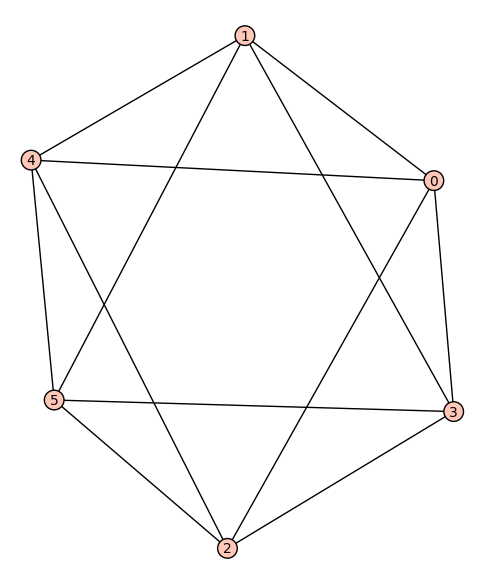
\includegraphics[width=0.45\linewidth]{q3}}
%\caption{Generic layout}
%\end{subfigure}%
%\begin{subfigure}[b]{0.4\linewidth}
\subfloat[][Planar layout]
{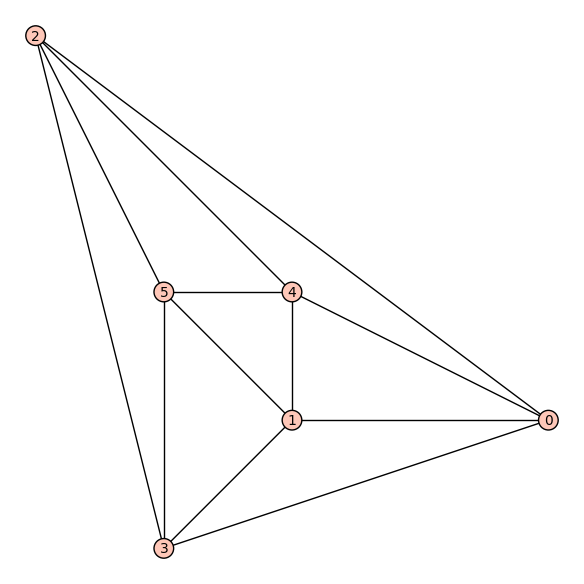
\includegraphics[width=0.5\linewidth]{q3_planar}}
%\caption{Planar layout}
%\end{subfigure}%
%\begin{subfigure}[b]{0.4\linewidth}
\subfloat[][Circular layout]
{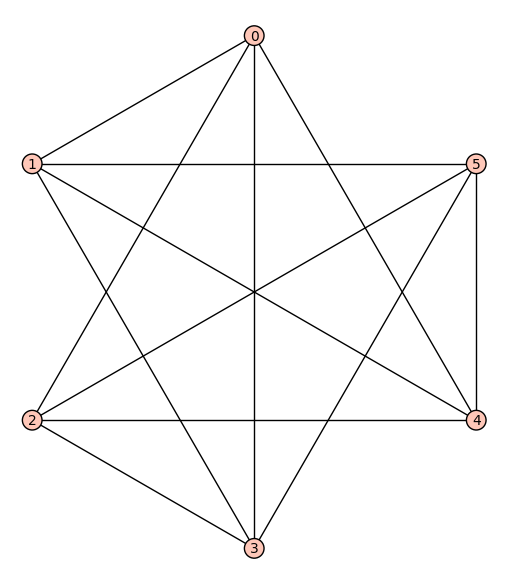
\includegraphics[width=0.5\linewidth]{q3_circularr}}
%\caption{Circular layout}
%\end{subfigure}
\caption{Different layouts for ${\text{X}}_3(2,1)$}
\end{figure*}
\begin{figure*}[!h]
\centering
%\hspace*{-1.5cm}
%\begin{subfigure}[b]{0.5\linewidth}
\subfloat[][Default layout]
{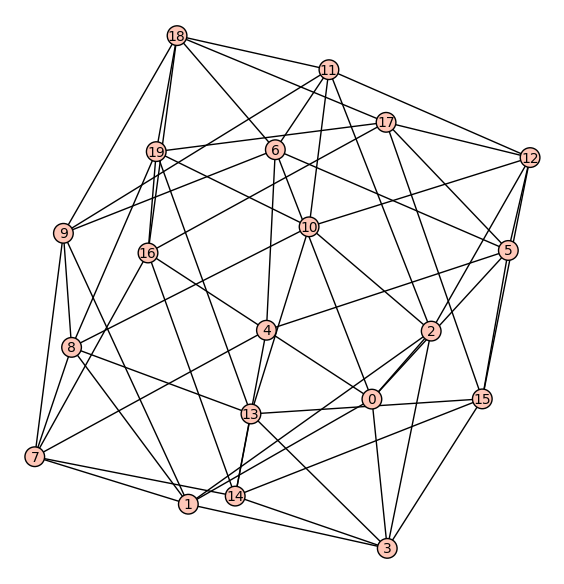
\includegraphics[width=0.45\linewidth]{q5_a2_d2}}
%\caption{Default layout}
%\end{subfigure}%
%\begin{subfigure}[b]{0.45\linewidth}
\subfloat[][Circular layout]
{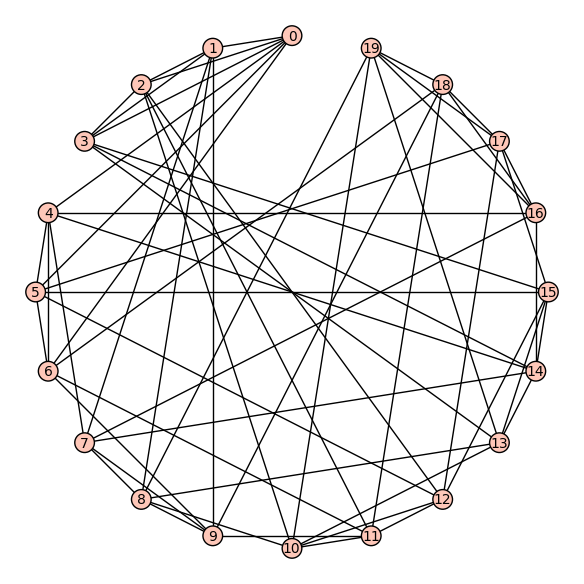
\includegraphics[width=0.45\linewidth]{q5_a2_d2_circular}}
%\caption{Circular layout}
%\end{subfigure}%
\caption{Different layouts for ${\text{X}}_5(2,2)$}
\end{figure*}
%(qui ci vanno gli esempi, sia ripresi dal libro che no)
%(ci sono altre osservazioni carine sulle similutini col caso continuo, ma dovrei studiarci bene e non so se c'è spazio)


\begin{theorem}\label{important}
Let $q=p^r$ , where $p$ is an odd prime. Let $0\neq a\in \F_q$, and let $\delta \in \F_q$ be a non square element.
Then the following holds:
\begin{itemize}
\item[1.] if $a\neq 4\delta$ then the graph is $(q+1)-regular$;
\item[2.] if $0\neq c\in \F_q$ then the graphs $\xq a$ and $X_q(\delta c^2, a c^2)$ are isomorphic;  
\item[3.] $\forall 0 \leq s < r, s\in \N$ the graphs $\xq a$ and $X_q (\delta^{p^s}, a^{p^s})$ are isomorphic;
\item[4.] if $a\neq 4\delta$ then $\xq a$ is the Cayley graph for the group $\Aff q$ with generators:
\begin{equation}\label{generators}
	S_q(\delta,a) = \Big\{ \begin{pmatrix} y & x \\ 0 & 1 \end{pmatrix} \in \Aff q \colon x^2=ay+(y-1)^2 \delta \Big\};
\end{equation}
\item[5.] if $a\neq 4\delta$ then $\xq a$ is connected.
\end{itemize}


(ci sarebbe un altro punto, non mi sembra né utile né interessante, lo ometto per adesso)
\begin{proof}
1. WLOG I can assume $z=\rd$, because of the transitivity of the action and the invariance of the distance.
In fact, if $g \cdot \rd = z$, then 
\begin{equation*}
\lvert \{\bar{w} \colon \dist (\rd, \bar{w})=a\}\rvert=\lvert \{w \colon \dist (z,w)=a \} \rvert.
\end{equation*}
So we are interested in the solutions of the equation $\dist (\rd, z)=a$.

Suppose $z=x+y\rd$. Then
\begin{align} \label{distance}
	\dist (\rd, z)=a & \iff \Norm (\rd - z) = ay\\		\notag
					 & \iff (\rd - z)\overline{(\rd - z)}=ay\\ \notag
					 & \iff (-x+(1-y)\rd)(-x-(1-y)\rd )=ay\\   \notag
					 & \iff x^2 = ay + (y-1)^2 \delta. 
\end{align}
We must be careful: if $z$ is a solution of the previous equation, we must check that $z\in H_q$, that is $y\neq 0$.
But this is always true: if $y=0$ from the previous equation we obtain $\delta=(x(y-1)^{-1})^2$,
but this is impossible, since $\delta$ is a non square element.
So we can simply find solutions of $\Norm (\rd - z) = ay$ in $\F_{q^2}$, and they will belong to $H_q$ as well.

We recall (see \cite{lidl1994introduction}) that $\mathfrak{N}\colon \F_{q^2}^{*} \to \F_q^{*}$ is an onto group omomorphism.
We want to use this property to find the number of solutions of $\Norm (\rd - z) = ay$:
\begin{equation}
	\lvert \mathfrak{N}^{-1}(a)\rvert=\frac{\abs {\F_{q^2}^{*}}}{\abs {\F_q^{*}}}=\frac{q^2+1}{q-1}=q+1.
\end{equation}
Fix $c=(\frac{a}{2\delta}-1)\rd$ and $d=(1-\frac{a}{4\delta})a$. Then:
\begin{align*}
	\Norm (z+c) = d &\iff (z+c)(\bar{z}+\bar{c})=d \\
					&\iff ((z-\rd)+\frac{a}{2\delta})((\bar{z}+\rd)-\frac{a}{2\delta})=(1-\frac{a}{4\delta})a \\
					&\iff (z-\rd)(\bar{z}+\rd)+(\frac{a}{2\delta})(\bar{z}+\delta-z+\delta)+\frac{a^2}{4\delta}=a-\frac{a^2}{4\delta} \\
					&\iff \Norm (z-\rd)+(\frac{a}{2\delta})(-2y\rd +2\rd)=a \iff \Norm (z - \rd) = ay.
\end{align*}
So, if we set $w=z+c$, in the case $d\neq 0$, I can find $q+1$ solutions in $\F_{q^2}^{*}$ of $\Norm w = d$.
But $d=0 \iff a=0,4\delta$, cases that are excluded by hypothesis.
(il libro fa altre considerazioni oer concludere che il numero di soluzioni è precisamente q+1, a me pare suff così per concludere).

Hence the equation $\dist (\rd, z)=a$ has exactly $q+1$ solutions, that is the graph is $(q+1)-regular$.

2. We first notice that that $\delta c^2$ is a non square element, so the definition of the graph $X_q(\delta c^2, a c^2)$
is well posed. Clearly multiplying by $c^2$ is a bijection of $H_q$ to itself, so the vertexes of the two graphs are the same.

In the definition of $\Norm z = z \bar{z}$ seems that the choice of $\rd$ matters; but as we already noticed $\bar{z}=z^q$.
This means that $\Norm z = z z^q$ is independent from the choice of $\rd$. The same does not hold for the imaginary part:
if $z=x+y\rd$, then $z=x+yc^{-1} c \rd $. So, with an obvious notation, 
\begin{equation} \label{ims}
	\Im_{c\rd} (z) = c^{-1} \Im_{\rd} (z).
\end{equation}
What we need to prove can be stated as follows:
\begin{equation*}
	\frac{\Norm (z-w)}{\Im_{\rd} (z) \Im_{\rd} (w)}=\dist_{\rd} (z,w)=a \iff 
	\frac{\Norm (z-w)}{\Im_{c\rd} (z) \Im_{c\rd} (w)}=\dist_{c\rd} (z,w)=ac^2.
\end{equation*}
But this is easy thanks to \ref{ims}:
\begin{align*}
	\frac{\Norm (z-w)}{\Im_{c\rd} (z) \Im_{c\rd} (w)}=ac^2 &\iff \frac{\Norm (z-w)}{c^{-1}\Im_{\rd} (z)c^{-1} \Im_{\rd} (w)}=ac^2 \\
															&\iff \frac{\Norm (z-w)}{\Im_{\rd} (z) \Im_{\rd} (w)}=a.
\end{align*}

3. We can restrict the proof to the case $s=1$, the general statement follows by induction.
Raising to $p$ is a field automorphisim, hence non square elements are mapped into non square elements 
and it is a bijection from $H_q$ to itself. So the graph $X_q (\delta^{p}, a^{p})$ is well defined and the vertexes of 
$\xq a$ and $X_q (\delta^{p}, a^{p})$ are the same. We observe in particular that $(x+y\rd)^p=x^p+y^p\rd^p$.
Moreover, using a notation similar to the previous point,
\begin{align*}
	\dist_{\rd} (z,w)=a & \iff \frac{\Norm (z-w)}{\Im_{\rd} (z) \Im_{\rd} (w)}=a\\
	& \iff (\frac{\Norm (z-w)}{\Im_{\rd} (z) \Im_{\rd} (w)})^p = a^p \\
	& \iff \frac{\Norm ((z-w)^p)}{\Im_{\rd^p} (z^p) \Im_{\rd^p} (w^p)}=a^p\\
	& \iff \frac{\Norm (z^p-w^p)}{\Im_{\rd^p} (z^p) \Im_{\rd^p} (w^p)}=a^p \iff \dist_{\rd^p} (z^p,w^p)=a^p,
\end{align*}
and we conclude that the two graphs are isomorphic.

4. In the statement we identify $H_q$ and $\Aff q$ by the bijection given by the action on the point $\rd$:
$x+y\rd \leftrightarrow \begin{pmatrix} y & x \\ 0 & 1 \end{pmatrix}$.
Suppose $S_q(\delta,a)$ as in \ref{generators}. We notice that the equation in the definition of $S_q(\delta,a)$
is the same as in \ref{distance}. So we obtain $s \in S_q(\delta,a) \iff \dist (\rd, s \cdot \rd) = a$. Moreover
\begin{align*}
	g,h \in \Aff q \quad \text{are adjacent} &\iff \dist (h \cdot \rd, g \cdot \rd) = a \iff \dist ( \rd, h^{-1}g \cdot \rd) = a\\
	&\iff h^{-1}g \in S_q(\delta,a) \iff \exists \, s \in S_q(\delta,a)\colon g=hs,
\end{align*}
so $S_q(\delta,a)$ is a set of generators for the graph. We only need to check that it is closed under inversion (our graph is undirected):
but this follows from the fact that $\dist(\rd, s\cdot \rd)=\dist(s^{-1}\rd, s^{-1}s\cdot \rd)=\dist(\rd, s^{-1}\cdot \rd)$.
Hence $\xq a$ is a Cayley graph with generators $S_q(\delta,a)$.

5. I want to prove that $S_q(\delta,a)$ generates $\Aff q$, that is every $g \in \Aff q$ can be expressed by the product
of a finite number of elements of $S_q(\delta,a)$. We first observe that
\begin{equation}\label{gatto}
	\begin{pmatrix} a & b \\ 0 & 1 \end{pmatrix}=\begin{pmatrix} 1 & b \\ 0 & 1 \end{pmatrix} \begin{pmatrix} a & 0 \\ 0 & 1 \end{pmatrix},
\end{equation}
so it enough to show that $\forall a,b \in \F_q^{*}$ the matrices 
$\begin{pmatrix} 1 & b \\ 0 & 1 \end{pmatrix}$ and $\begin{pmatrix} a & 0 \\ 0 & 1 \end{pmatrix}$
belongs to the subgroup generated by $S_q(\delta,a)$.

Now, since $\vert S_q(\delta,a)\vert=q+1$ (this is because its cardinality is exactly the number of points adjacent to $\rd$,
 and in the case $a\neq 4\delta$ the graph is $q+1$ regular), we have that:
 \begin{equation}\label{elem}
 	\exists x,y \in \F_q^{*} \colon g = \begin{pmatrix} y & x \\ 0 & 1 \end{pmatrix} \in S_q(\delta,a).
 \end{equation}

Let $\alpha$ be a generator of $\F_q^{*}$. Then $y=\alpha^e$ for some $e\in {1, \dots , q-1}.$ Thus we proved that
$E=\big\{ e \in \{1, \dots , q-1\} \colon \exists x \in \F_q^{*} \text{ with } \begin{pmatrix} \alpha^e & x \\ 0 & 1 \end{pmatrix} \in S_q(\delta,a) \big\} \neq \emptyset$.
Define $t$ as the g.c.d. of the elements of $E$
($e\in E \Rightarrow e=kt \text{ for some } k \in \N^{+}$). We want to prove that $t=1$.

We define the map
\begin{align*}
	\phi \colon & S_q(\delta,a) \longrightarrow \{kt \colon k in \{1, \dots ,\frac{q-1}{t}\}\}\\
				&  \begin{pmatrix} \alpha^e & x \\ 0 & 1 \end{pmatrix} \longmapsto e.
\end{align*}
The map is well defined by definition of $t$.
We notice that
\begin{equation}\label{double}
\begin{pmatrix} y & x \\ 0 & 1 \end{pmatrix} \in S_q(\delta,a) \Rightarrow \begin{pmatrix} y & -x \\ 0 & 1 \end{pmatrix} \in S_q(\delta,a)
\end{equation}
by definition of $S_q(\delta,a)$. So we have that
$\forall e \in \{kt \colon k in \{1, \dots ,\frac{q-1}{t}\}\} \,\, \vert \phi^{-1}(e)\vert \le 2$, and we observe that:
\begin{equation*}
	q+1 = \vert S_q(\delta,a)\vert = \vert \bigsqcup_{k=1}^{\frac{q-1}{t}} \phi^{-1}(kt) \vert \le \frac{2(q-1)}{t}.
\end{equation*}
The previous equation implies $t=1$.
Suppose $E={e_1,\dots, e_s}$. Then we have proved that $\exists a_i \in Z \colon \sum_{i=1}^s a_i e_i =t$, and so
\begin{equation}
	\begin{pmatrix} \alpha^{e_1} & x_1 \\ 0 & 1 \end{pmatrix}^{a_1} \dots 
	\begin{pmatrix} \alpha^{e_s} & x_s \\ 0 & 1 \end{pmatrix}^{a_s}=
	\begin{pmatrix} \alpha^{\sum_{i=1}^s a_i e_i} & * \\ 0 & 1 \end{pmatrix}=
	\begin{pmatrix} \alpha & * \\ 0 & 1 \end{pmatrix}^{a_s}
\end{equation}
 belongs to $\langle S_q(\delta,a) \rangle$. Hence $\forall y \in \F_q^{*}\, \exists x \in \F_q \colon 
 \begin{pmatrix} y & x \\ 0 & 1 \end{pmatrix} \in \langle S_q(\delta,a) \rangle$. 

Now, let $g,x,y$ be as in \ref{elem}. Then by \ref{double}:
\begin{align*}
	g \in S_q(\delta,a) &\Rightarrow g^{-1}= \begin{pmatrix} y^{-1} & -y^{-1}x \\ 0 & 1 \end{pmatrix} \in S_q(\delta,a)
	\Rightarrow \begin{pmatrix} y^{-1} & y^{-1}x \\ 0 & 1 \end{pmatrix} \in S_q(\delta,a)\\ &\Rightarrow h=
	\begin{pmatrix} y & x \\ 0 & 1 \end{pmatrix}\begin{pmatrix} y^{-1} & y^{-1}x \\ 0 & 1 \end{pmatrix}=
	\begin{pmatrix} 1 & 2x \\ 0 & 1 \end{pmatrix} \in \langle S_q(\delta,a) \rangle.
\end{align*}
We notice that $2x\neq 0$. Let $b \in \F_q^{*}$ and let $\bar{y}=\frac{2x}{b}\neq 0$. We proved that
$\exists \bar{x} \colon  \bar{h}=\begin{pmatrix} \bar{y} & \bar{x} \\ 0 & 1 \end{pmatrix} \in \langle S_q(\delta,a) \rangle$.
Hence $\bar{h}^{-1} h \bar{h} = \begin{pmatrix} 1 & b \\ 0 & 1 \end{pmatrix}\in \langle S_q(\delta,a) \rangle$.

If we remember \ref{gatto}, the only thing left to prove is that $\forall a\in \F_q^{*}, \,\begin{pmatrix} a & 0 \\ 0 & 1 \end{pmatrix}\in \langle S_q(\delta,a) \rangle$. Let $c\in \F_q$ be such that $\begin{pmatrix} a & c \\ 0 & 1 \end{pmatrix}\in \langle S_q(\delta,a) \rangle$. Then
\begin{equation*}
	\begin{pmatrix} a & 0 \\ 0 & 1 \end{pmatrix} = \begin{pmatrix} 1 & -c \\ 0 & 1 \end{pmatrix} \begin{pmatrix} a & c \\ 0 & 1 \end{pmatrix} \in \langle S_q(\delta,a) \rangle,
\end{equation*}
and this (finally) completes the proof.
\end{proof}
\end{theorem}

Now we are interested in finding properties of these graphs, and of course we are interested in its adjacency matrix.
\begin{defn}
	Given a character $\chi$ of $\F_q^{*}$, we define th \emph{finite power function} $p_{\chi}$:
	\begin{align*}
		p_{\chi} \colon H_q & \longrightarrow \C \\
		z & \longmapsto p_{\chi}(z)=\chi (\Im z).
	\end{align*}
\end{defn}
We are interested in these functions because they are eigenfunctions of our graphs, as the following proposition shows.
\begin{prop}
Let $A$ be the adjacency matrix of our graph $\xq a$. Then for all characters $\chi$, the function $p_{\chi}$
defined above is an eigenfunction for $A$. Moreover their eigenvalues are explicitly:
\begin{equation}\label{eigen}
	\lambda_{chi}=\sum_{w\in S_q(\delta,a)} \chi (\Im w).
\end{equation}
\begin{proof}
By theorem \ref{important} we recall that our graph is a Cayley one, so two vertexes are connected by an edge if and only if
we can obtain one from the other multiplying by an element of the sets of generators.
So we have by definition of adjacency operator:
\begin{align*}
	Ap_{\chi}(\begin{pmatrix} y & x \\ 0 & 1 \end{pmatrix} \delta) &=
	 \sum_{\begin{pmatrix} v & u \\ 0 & 1 \end{pmatrix} \in S_q(\delta,a)} p_{\chi}(\begin{pmatrix} v & u \\ 0 & 1 \end{pmatrix}
	 \begin{pmatrix} y & x \\ 0 & 1 \end{pmatrix} \delta)=\\
	 &=\sum_{\begin{pmatrix} v & u \\ 0 & 1 \end{pmatrix} \in S_q(\delta,a)} \chi (\Im (\begin{pmatrix} v & u \\ 0 & 1 \end{pmatrix}
	 \begin{pmatrix} y & x \\ 0 & 1 \end{pmatrix} \delta))=\\
	 &=\sum_{\begin{pmatrix} v & u \\ 0 & 1 \end{pmatrix} \in S_q(\delta,a)}\chi (vy)=\\
	 &=(\sum_{\begin{pmatrix} v & u \\ 0 & 1 \end{pmatrix} \in S_q(\delta,a)}\chi (\Im \begin{pmatrix} v & u \\ 0 & 1 \end{pmatrix}))\chi (\Im  \begin{pmatrix} y & x \\ 0 & 1 \end{pmatrix})=\\
	 &=\lambda_{\chi} p_{\chi} (\begin{pmatrix} y & x \\ 0 & 1 \end{pmatrix} \delta).
\end{align*}
\end{proof}
\end{prop}We could have simply seen this as a consequence of (mettere qui ref a roba su rapp di aff), which proves that the eigenvalues are one dimensional.

We are interested in bounds on the absolute value of \ref{eigen}, to see for instance that the graph is Ramanujan. 
To find these bounds we need some more advanced theory of finite fields: we will follow \cite{schmidt1976equations},
giving results and only sketches of the proofs for shortness.
\begin{defn}
Let $\K$ be a field and $\F$ a subfield. We say that $\K$ is an \emph{algebraic extension} of $\F$ if
$\forall k \in \K \, \exists f(x) \in \F[x] \colon f(k)=0$.
\end{defn}
\begin{defn}
$f(x,y)\in \F_q[x,y]$ is said \emph{absolutely irreducible} if it is irreducible over $\F_q$ and over all its algebraic extensions.
\end{defn}
The following lemma will be useful later.

\begin{lemma}\label{tre}
	Let $y^d-f(x)\in \K[x,y]$. Then the following conditions are equivalent:
	\begin{itemize}
	\item[1.] $y^d-f(x)$ is absolutely irreducible;
	\item[2.] $y^d-cf(x)$ is absolutely irreducible for every $c \in \K^{*}$;
	\item[3.] if $f(x)=a \prod_{i=1}^s (x-\alpha_i)^{d_i}, \, \alpha_i \neq \alpha_j$ is the factorization of $f(x)$ over
	 its algebraic closure $\bar{\K}$, then $\gcd(d_1,\dots ,d_s)=1$.
	\end{itemize}
\begin{proof} We will give only a sketch of the proof.

$1. \Rightarrow 2.$ Just observe that $y^d-cf(x)=c(z-f(x)),\, z=\frac{y}{\sqrt[d]{c}}$.

$2. \Rightarrow 3.$ Let $t=\gcd(d_1,\dots ,d_s)$. By contradiction suppose $t > 1$.
Define $g(x)=a \prod_{i=1}^s (x-\alpha_i)^{d_i/t}$. Then $y^{d/t}-g(x)$ divides $y^d-\frac{1}{a}f(x)=y^d-\frac{1}{a}g(x)^t$,
against the hypothesis.

$3. \Rightarrow 1.$ We will denote by $\L=\bar{\K}(x)$ the field of fractions in one variable.
We will see $y^d-f(x) \in \L[y]$.
In $\bar{\K}[x]$ factorize $y^d-1=\prod_{i=1}^d (y-\beta_i)$.  .
Then in the algebraic closure $\bar{L}$ of $L$ we have $y^d-f(x)=\prod_{i=1}^{s}(y-\beta_i \eta)$,
where $\eta \in \bar{\L}$ is an arbitrary root of $y^d-f(x)$.
Then by contrary we suppose that $y^d-f(x)$ is reducible. Let $l$ be the minimum positive integer such that
$\eta^l=h(x)\in \bar{K}[x]$. Then, using the fact that $\eta^d=f(x)$, we see that $f(x)=h(x)^{d/l}$, against the hypothesis. 
\end{proof}
\end{lemma}
In the following if will be  convenient to extend the definition of characters $\chi$ of $\F_q^{*}$
to 0 in the following way:
\begin{equation*}
	\chi (0)=\begin{cases}&1\quad \text{if $\chi$ is the trivial character}\\ &0 \quad\text{otherwise} \end{cases}.
\end{equation*}

Now we can state a theorem, whose corollary is the bound we need.
\begin{theorem}
Let $\chi$ be a (non trivial) character of $\F_q{*}$, and let $d$ be its order. Let $f(x) \in \F_q[x]$ have exactly
$m$ distinct zeros, and suppose that $y^d-f(x)$ is absolutely irreducible. Then:
\begin{equation}
	\vert \sum_{xa \in \F_q} \chi (f(a)) \vert=(m-1)\sqrt{q}. 
\end{equation}
\begin{proof}
	See \cite{•}.
\end{proof}
\end{theorem}

\begin{cor}
	The one dimensional eigenvalues of the adjacency operator of $\xq a$ satisfy the Ramanujan bound, that is:
\begin{equation*}
	\vert \lambda_{\chi} \vert \le 2\sqrt{q}.
\end{equation*}
\begin{proof}
	Define $\epsilon$ as the quadratic character on $\F_q$:
\begin{equation*}
	\epsilon (x)=\begin{cases}&1 \quad \text{if $x$ is a square}\\ -&1 \quad \text{if $x$ is a non square}\\ &0 \quad x=0 \end{cases}.
\end{equation*}
Let $g(y)=ay+(y-1)^2 \delta$ and $w=x+y\rd$. Then
\begin{equation}\label{equivalence}
w \in S_q(\delta,a) \iff x^2=g(y) \iff g(y) \text{is a square and} x \text{is one of its roots}.
\end{equation}
In particular if $g(y)=0$ then $x=0$ (only $1=\epsilon(0)+1$ solution), while if $g(y)\neq 0$ and $g(y)$ is a square then we have
$2=\epsilon (g(y)+1)$; if $g(y)\neq 0$ and $g(y)$ is a non square then we have $0=\epsilon (g(y)+1$ solutions.

By the previous observation and by \ref{equivalence} we get:
\begin{equation}
\lambda_{chi}=\sum_{y \in \F_q} \chi (y)(\epsilon(g(y))+1)=(\lambda_{chi}=
\sum_{y \in \F_q}\chi (y)\epsilon(g(y)))+(\lambda_{chi}\chi (y)).
\end{equation}
The second sum is equal to zero due to the orthogonality of the characters (aggiungere ref).
We have reached a form similar to the previous theorem: we need only to express the two different characters in a common form.

But the characters of a cyclic group form a cyclic group of the same order ($q-1$ in our case). So let $\eta$ be a generator character.
Then, if $d$ is the order of $\chi$, then we can write $\chi=\eta^{\frac{q-1}{d}}$ and $\epsilon=\eta^{\frac{q-1}{2}}$
(since the order of $\epsilon$ is trivially 2). Hence we have:
\begin{equation}
	\lambda_{\chi}=\sum_{y \in \F_q} \eta^{\frac{q-1}{d}}(y)\eta^{\frac{q-1}{2}}(g(y))=\lambda_{\chi}=\sum_{y \in \F_q}
	\eta^m(y^{\frac{q-1}{md}}g(y)^{\frac{q-1}{2m}}),
\end{equation}
where $m=\gcd(\frac{q-1}{d},\frac{q-1}{2})$. We want to use point 3. of lemma \ref{tre} to prove that $z^{\frac{q-1}{m}}-f(y)$
is absolutely irreducible, where $f(y)=y^{\frac{q-1}{md}}g(y)^{\frac{q-1}{2m}}$ and $\frac{q-1}{m}$ is trivially the order
of $\eta^m$. Now, $g(y)=\delta y^2+(a-2\delta)y+\delta$
and its discriminant is $a(a-4\delta)$. Since $a\neq 0, 4\delta$ by hypothesis then its roots are non zero
and distinct, say $\alpha_1. \alpha_2$. Hence $f(y)$ has 3 distinct roots $0,\alpha_1,\alpha_2$ with multiplicity 
$\frac{q-1}{md}, \frac{q-1}{2m},\frac{q-1}{2m}$ respectively.
Looking at point 3. of the lemma, we see that we must prove that $r=\gcd(\frac{q-1}{m},\frac{q-1}{md},\frac{q-1}{2m})=1$.
But this is true because $r\vert \gcd(\frac{q-1}{md},\frac{q-1}{2m})=1$, where the last equality holds by definition of $m$.
So the polynomial $z^{\frac{q-1}{m}}-f(y)$ is absolutely irreducible by the lemma and the bound we where looking holds 
by the previous theorem.
\end{proof}
\end{cor}


\printbibliography
\end{document}
